\subsection{最小生成树}
\begin{frame}\ft{\subsecname}
  \begin{small}
\begin{wenti}
如图所示的九个村庄,想架设通信网络,如何以最小的成本完成设计?
\end{wenti}	
\begin{figure}
\centering
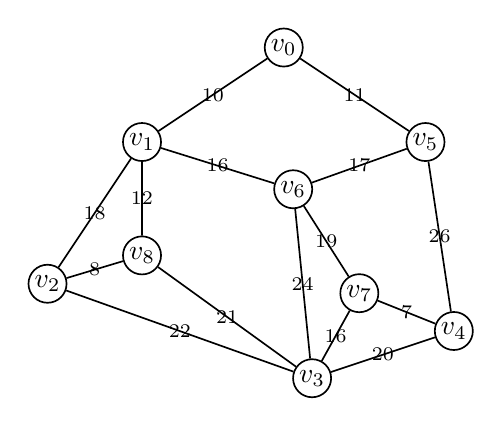
\begin{tikzpicture}[scale=1.2,node distance=2cm,semithick,inner sep=1pt,bend angle=45]
%\draw[help lines] (-3,-3) grid (3,0);
\node[circle,draw] (v0)  at (0,0)   {$v_0$};
\node[circle,draw] (v5)  at (1.5,-1) {$v_5$};
\node[circle,draw] (v1) at (-1.5,-1) {$v_1$};
\node[circle,draw] (v2)  at (-2.5,-2.5)   {$v_2$};
\node[circle,draw] (v8)  at (-1.5,-2.2) {$v_8$};
\node[circle,draw] (v6)  at (0.1,-1.5) {$v_6$};
\node[circle,draw] (v3)  at (0.3,-3.5) {$v_3$};
\node[circle,draw] (v7)  at (0.8,-2.6) {$v_7$};
\node[circle,draw] (v4)  at (1.8,-3.0) {$v_4$};
%%
\path
(v0) edge node{\scriptsize $10$} (v1)
     edge node{\scriptsize $11$} (v5)
(v1) edge node{\scriptsize $18$} (v2)
     edge node{\scriptsize $16$} (v6)
     edge node{\scriptsize $12$} (v8)
(v2) edge node{\scriptsize $8$} (v8)
     edge node{\scriptsize $22$} (v3)
(v3) edge node{\scriptsize $21$} (v8)
     edge node{\scriptsize $24$} (v6)
     edge node{\scriptsize $16$} (v7)
     edge node{\scriptsize $20$} (v4)
(v4) edge node{\scriptsize $7$} (v7)
     edge node{\scriptsize $26$} (v5)
(v5) edge node{\scriptsize $17$} (v6)
(v6) edge node{\scriptsize $19$} (v7);                     
\end{tikzpicture}

\end{figure}
%\pause

所谓最小成本,就是用$n$个顶点,$n-1$条边把一个连通图连接起来,并使得权值的和最小。
    
  \end{small}
\end{frame}

\begin{frame}\ft{\subsecname}
\begin{figure}
\centering
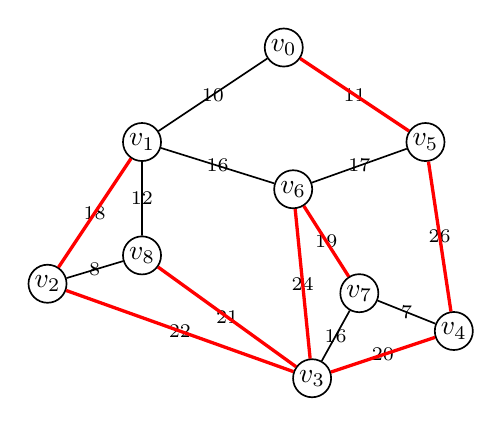
\begin{tikzpicture}[scale=1.2,node distance=2cm,semithick,inner sep=1pt,bend angle=45]
%\draw[help lines] (-3,-3) grid (3,0);
\node[circle,draw] (v0)  at (0,0)   {$v_0$};
\node[circle,draw] (v5)  at (1.5,-1) {$v_5$};
\node[circle,draw] (v1) at (-1.5,-1) {$v_1$};
\node[circle,draw] (v2)  at (-2.5,-2.5)   {$v_2$};
\node[circle,draw] (v8)  at (-1.5,-2.2) {$v_8$};
\node[circle,draw] (v6)  at (0.1,-1.5) {$v_6$};
\node[circle,draw] (v3)  at (0.3,-3.5) {$v_3$};
\node[circle,draw] (v7)  at (0.8,-2.6) {$v_7$};
\node[circle,draw] (v4)  at (1.8,-3.0) {$v_4$};
%%
\path
(v0) edge node{\scriptsize $10$} (v1)
     edge node{\scriptsize $11$} (v5)
(v1) edge node{\scriptsize $18$} (v2)
     edge node{\scriptsize $16$} (v6)
     edge node{\scriptsize $12$} (v8)
(v2) edge node{\scriptsize $8$} (v8)
     edge node{\scriptsize $22$} (v3)
(v3) edge node{\scriptsize $21$} (v8)
     edge node{\scriptsize $24$} (v6)
     edge node{\scriptsize $16$} (v7)
     edge node{\scriptsize $20$} (v4)
(v4) edge node{\scriptsize $7$} (v7)
     edge node{\scriptsize $26$} (v5)
(v5) edge node{\scriptsize $17$} (v6)
(v6) edge node{\scriptsize $19$} (v7);  

\draw[very thick,red]  (v0)--(v5)--(v4)--(v3)--(v2)--(v1);    
\draw[very thick,red]  (v3)--(v8) (v3)--(v6)--(v7);                               
\end{tikzpicture}

\caption{方案一:$11+26+20+22+18+21+24+19=161$}
\end{figure}
\end{frame}

\begin{frame}\ft{\subsecname}
\begin{figure}
\centering
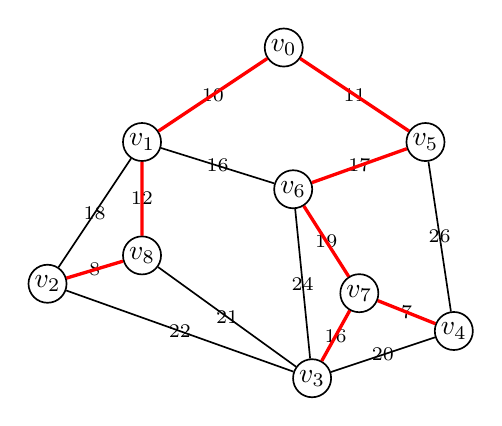
\begin{tikzpicture}[scale=1.2,node distance=2cm,semithick,inner sep=1pt,bend angle=45]
%\draw[help lines] (-3,-3) grid (3,0);
\node[circle,draw] (v0)  at (0,0)   {$v_0$};
\node[circle,draw] (v5)  at (1.5,-1) {$v_5$};
\node[circle,draw] (v1) at (-1.5,-1) {$v_1$};
\node[circle,draw] (v2)  at (-2.5,-2.5)   {$v_2$};
\node[circle,draw] (v8)  at (-1.5,-2.2) {$v_8$};
\node[circle,draw] (v6)  at (0.1,-1.5) {$v_6$};
\node[circle,draw] (v3)  at (0.3,-3.5) {$v_3$};
\node[circle,draw] (v7)  at (0.8,-2.6) {$v_7$};
\node[circle,draw] (v4)  at (1.8,-3.0) {$v_4$};
%%
\path
(v0) edge node{\scriptsize $10$} (v1)
     edge node{\scriptsize $11$} (v5)
(v1) edge node{\scriptsize $18$} (v2)
     edge node{\scriptsize $16$} (v6)
     edge node{\scriptsize $12$} (v8)
(v2) edge node{\scriptsize $8$} (v8)
     edge node{\scriptsize $22$} (v3)
(v3) edge node{\scriptsize $21$} (v8)
     edge node{\scriptsize $24$} (v6)
     edge node{\scriptsize $16$} (v7)
     edge node{\scriptsize $20$} (v4)
(v4) edge node{\scriptsize $7$} (v7)
     edge node{\scriptsize $26$} (v5)
(v5) edge node{\scriptsize $17$} (v6)
(v6) edge node{\scriptsize $19$} (v7);  

\draw[very thick,red]  (v0)--(v5)--(v6)--(v7)--(v3) (v7)--(v4) (v0)--(v1)--(v8)--(v2);    
\end{tikzpicture}

\caption{方案二:$8+12+10+11+17+19+16+7=100$}
\end{figure}
\end{frame}

\begin{frame}\ft{\subsecname}
\begin{figure}
\centering
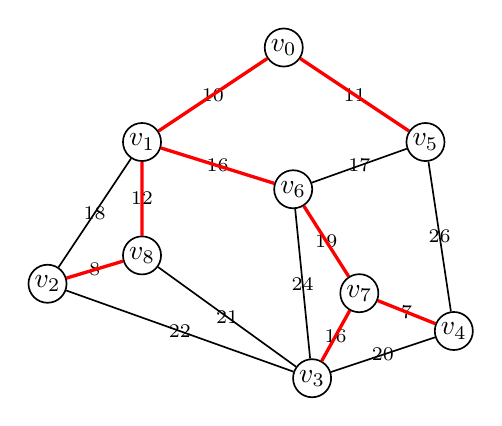
\begin{tikzpicture}[scale=1.2,node distance=2cm,semithick,inner sep=1pt,bend angle=45]
%\draw[help lines] (-3,-3) grid (3,0);
\node[circle,draw] (v0)  at (0,0)   {$v_0$};
\node[circle,draw] (v5)  at (1.5,-1) {$v_5$};
\node[circle,draw] (v1) at (-1.5,-1) {$v_1$};
\node[circle,draw] (v2)  at (-2.5,-2.5)   {$v_2$};
\node[circle,draw] (v8)  at (-1.5,-2.2) {$v_8$};
\node[circle,draw] (v6)  at (0.1,-1.5) {$v_6$};
\node[circle,draw] (v3)  at (0.3,-3.5) {$v_3$};
\node[circle,draw] (v7)  at (0.8,-2.6) {$v_7$};
\node[circle,draw] (v4)  at (1.8,-3.0) {$v_4$};
%%
\path
(v0) edge node{\scriptsize $10$} (v1)
     edge node{\scriptsize $11$} (v5)
(v1) edge node{\scriptsize $18$} (v2)
     edge node{\scriptsize $16$} (v6)
     edge node{\scriptsize $12$} (v8)
(v2) edge node{\scriptsize $8$} (v8)
     edge node{\scriptsize $22$} (v3)
(v3) edge node{\scriptsize $21$} (v8)
     edge node{\scriptsize $24$} (v6)
     edge node{\scriptsize $16$} (v7)
     edge node{\scriptsize $20$} (v4)
(v4) edge node{\scriptsize $7$} (v7)
     edge node{\scriptsize $26$} (v5)
(v5) edge node{\scriptsize $17$} (v6)
(v6) edge node{\scriptsize $19$} (v7);  

\draw[very thick,red]  (v0)--(v5) (v0)--(v1)--(v8)--(v2) (v1)--(v6)--(v7)--(v3) (v7)--(v4);    
\end{tikzpicture}

\caption{方案三:$8+12+10+11+16+19+16+7=99$}
\end{figure}
\end{frame}

\subsubsection{\tf Prim算法}
\begin{frame}\ft{\subsubsecname}
\tf Prim算法以某顶点为起点,逐步找各顶点上最小权值的边来构建最小生成树。
\end{frame}

\begin{frame}\ft{\subsubsecname}
\begin{figure}
\centering
\begin{tikzpicture}[scale=1,node distance=2cm,semithick,inner sep=1pt,bend angle=45]
%\draw[help lines] (-3,-3) grid (3,0);
\node[circle,draw] (v0)  at (0,0)   {$v_0$};
\node[circle,draw] (v5)  at (1.5,-1) {$v_5$};
\node[circle,draw] (v1) at (-1.5,-1) {$v_1$};
\node[circle,draw] (v2)  at (-2.5,-2.5)   {$v_2$};
\node[circle,draw] (v8)  at (-1.5,-2.2) {$v_8$};
\node[circle,draw] (v6)  at (0.1,-1.5) {$v_6$};
\node[circle,draw] (v3)  at (0.3,-3.5) {$v_3$};
\node[circle,draw] (v7)  at (0.8,-2.6) {$v_7$};
\node[circle,draw] (v4)  at (1.8,-3.0) {$v_4$};
%%
\path
(v0) edge node{\tiny $10$} (v1)
     edge node{\tiny $11$} (v5)
(v1) edge node{\tiny $18$} (v2)
     edge node{\tiny $16$} (v6)
     edge node{\tiny $12$} (v8)
(v2) edge node{\tiny $8$} (v8)
     edge node{\tiny $22$} (v3)
(v3) edge node{\tiny $21$} (v8)
     edge node{\tiny $24$} (v6)
     edge node{\tiny $16$} (v7)
     edge node{\tiny $20$} (v4)
(v4) edge node{\tiny $7$} (v7)
     edge node{\tiny $26$} (v5)
(v5) edge node{\tiny $17$} (v6)
(v6) edge node{\tiny $19$} (v7);  

\matrix (am) at (3.5,-1) [matrix of math nodes,left delimiter=(,right delimiter=),row sep=3pt,column sep=3pt,right] 
  {
    0 & 10& \infty & \infty & \infty & 11 & \infty & \infty & \infty\\
    10 & 0 & 18 & \infty & \infty & \infty & 16 & \infty & 12 \\
    \infty & \infty & 0 & 22 & \infty & \infty & \infty & \infty & 8\\
    \infty & \infty & 22 & 0 & 20 & \infty & \infty  & 16 & 21\\
    \infty & \infty & \infty & 20 & 0 & 26 & \infty & 7 & \infty\\
    11 & \infty & \infty & \infty & 26 & 0 & 17 & \infty & \infty\\
    \infty & 16 & \infty & \infty & \infty & 17 & 0 & 19 & \infty\\
    \infty & \infty & \infty & 16 & 7 & \infty & 19 & 0 & \infty\\
    \infty & 12 & 8 & 21 & \infty & \infty & \infty & \infty & 0\\
  };
  \node at (am-1-1) [above=10pt] {$v_0$}; 
  \node at (am-1-2) [above=10pt] {$v_1$};       
  \node at (am-1-3) [above=10pt] {$v_2$};       
  \node at (am-1-4) [above=10pt] {$v_3$};
  \node at (am-1-5) [above=10pt] {$v_4$};
  \node at (am-1-6) [above=10pt] {$v_5$};
  \node at (am-1-7) [above=10pt] {$v_6$};
  \node at (am-1-8) [above=10pt] {$v_7$};
  \node at (am-1-9) [above=10pt] {$v_8$};
  \node at (am-1-1) [left=18pt] {$v_0$}; 
  \node at (am-2-1) [left=18pt] {$v_1$};       
  \node at (am-3-1) [left=18pt] {$v_2$};       
  \node at (am-4-1) [left=18pt] {$v_3$};             
  \node at (am-5-1) [left=18pt] {$v_4$};
  \node at (am-6-1) [left=18pt] {$v_5$};       
  \node at (am-7-1) [left=18pt] {$v_6$};       
  \node at (am-8-1) [left=18pt] {$v_7$};             
  \node at (am-9-1) [left=18pt] {$v_8$};             

\end{tikzpicture}

\end{figure}
\end{frame}

\begin{frame}\ft{\subsubsecname}
  \begin{small}
\lstinputlisting[
language=c,
basicstyle=\ttfamily\scriptsize,
numbers=left,
numberstyle=\tiny,
xleftmargin=0.5em,
linerange={68-77},
frame=tb,
]{Chapters/Ch06/Code/adjmatrix/adjmatrix.c}
    
  \end{small}
\end{frame}

\begin{frame}\ft{\subsubsecname}
\lstinputlisting[
language=c,
basicstyle=\ttfamily\scriptsize,
numbers=left,
numberstyle=\tiny,
xleftmargin=0.5em,
linerange={78-96},
firstnumber=11,
frame=tb,
]{Chapters/Ch06/Code/adjmatrix/adjmatrix.c}
\end{frame}

\begin{frame}\ft{\subsubsecname}
\tf 创建两个一维数组lowcost和adjvtx,长度均为9。%\pause
\vspace{0.1in} 


\lstinputlisting[
language=c,
basicstyle=\ttfamily\scriptsize,
linerange={72-73},
]{Chapters/Ch06/Code/adjmatrix/adjmatrix.c}

\tf adjvtx[0]=0表示从顶点$v_0$开始,lowcost[0]=0表示$v_0$已被纳入到最小生成树中。 \vspace{0.1in} %\pause 

\tf注:之后凡是lowcost数值中的值被设置为0就表示此下标的顶点被纳入到最小生成树中。

\end{frame}

\begin{frame}[fragile]\ft{\subsubsecname}
\tf 
\lstinputlisting[
language=c,
basicstyle=\ttfamily\scriptsize,
linerange={74-77},
firstnumber=7,
numbers=left,
numberstyle=\tiny,
xleftmargin=0.5em,
]{Chapters/Ch06/Code/adjmatrix/adjmatrix.c}
读取邻接矩阵的第一行,赋值给lowcost,此时 
\begin{lstlisting}[xleftmargin=2em]
  0, 10,INF,INF,INF, 11,INF,INF,INF  (lowcost)
  0,  0,  0,  0,  0,  0,  0,  0,  0  (adjvtx)
\end{lstlisting}
 

\end{frame}


\begin{frame}[fragile]\ft{\subsubsecname}
\tf i=1 
\lstinputlisting[
language=c,
linerange={79-87},
basicstyle=\ttfamily\scriptsize,
firstnumber=12,
numbers=left,
numberstyle=\tiny,
xleftmargin=0.5em,
]{Chapters/Ch06/Code/adjmatrix/adjmatrix.c}
%\pause
执行前,
\begin{lstlisting}[xleftmargin=2em]
  0, 10,INF,INF,INF, 11,INF,INF,INF  (lowcost)
  0,  0,  0,  0,  0,  0,  0,  0,  0  (adjvtx)
\end{lstlisting} %\pause 
执行后,min=10,k=1,adjvtx[k]=0,打印结果为(0,1),表示边$(v_0,v_1)$为最小生成树的第一条边。
\end{frame}


\begin{frame}[fragile]\ft{\subsubsecname}

\begin{figure}
\centering
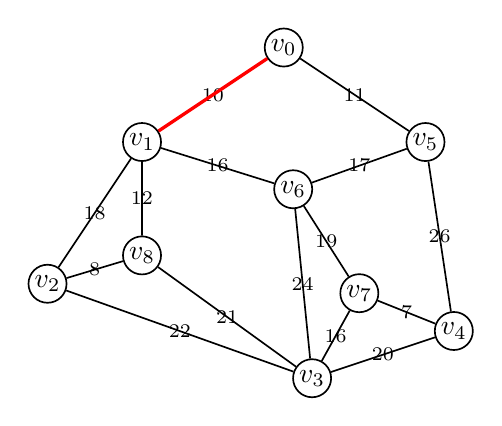
\begin{tikzpicture}[scale=1.2,node distance=2cm,semithick,inner sep=1pt,bend angle=45]
%\draw[help lines] (-3,-3) grid (3,0);
\node[circle,draw] (v0)  at (0,0)   {$v_0$};
\node[circle,draw] (v5)  at (1.5,-1) {$v_5$};
\node[circle,draw] (v1) at (-1.5,-1) {$v_1$};
\node[circle,draw] (v2)  at (-2.5,-2.5)   {$v_2$};
\node[circle,draw] (v8)  at (-1.5,-2.2) {$v_8$};
\node[circle,draw] (v6)  at (0.1,-1.5) {$v_6$};
\node[circle,draw] (v3)  at (0.3,-3.5) {$v_3$};
\node[circle,draw] (v7)  at (0.8,-2.6) {$v_7$};
\node[circle,draw] (v4)  at (1.8,-3.0) {$v_4$};
%%
\path
(v0) edge node{\scriptsize $10$} (v1)
     edge node{\scriptsize $11$} (v5)
(v1) edge node{\scriptsize $18$} (v2)
     edge node{\scriptsize $16$} (v6)
     edge node{\scriptsize $12$} (v8)
(v2) edge node{\scriptsize $8$} (v8)
     edge node{\scriptsize $22$} (v3)
(v3) edge node{\scriptsize $21$} (v8)
     edge node{\scriptsize $24$} (v6)
     edge node{\scriptsize $16$} (v7)
     edge node{\scriptsize $20$} (v4)
(v4) edge node{\scriptsize $7$} (v7)
     edge node{\scriptsize $26$} (v5)
(v5) edge node{\scriptsize $17$} (v6)
(v6) edge node{\scriptsize $19$} (v7);  

\draw[very thick,red](v0)--(v1);

\end{tikzpicture}

\end{figure}
\end{frame}

 

\begin{frame}[fragile]\ft{\subsubsecname}
\tf i=1 
\lstinputlisting[
language=c,
basicstyle=\ttfamily\scriptsize,
linerange={88-94},
firstnumber=21,
numbers=left,
numberstyle=\tiny,
xleftmargin=0.5em,
]{Chapters/Ch06/Code/adjmatrix/adjmatrix.c} %\pause 
 

执行前,k=1,
\begin{lstlisting}[xleftmargin=2em]
  0, 10,INF,INF,INF, 11,INF,INF,INF  (lowcost)
 10,  0, 18,INF,INF,INF, 16,INF, 12  (`第`v_1`行`)
  0,  0,  0,  0,  0,  0,  0,  0,  0  (adjvtx)
\end{lstlisting} %\pause 
执行后,
\begin{lstlisting}[xleftmargin=2em]
  0,  0, 18,INF,INF, 11, 16,INF, 12  (lowcost)
  0,  0,  1,  0,  0,  0,  1,  0,  1  (adjvtx)
\end{lstlisting}
\end{frame}

\begin{frame}[fragile]\ft{\subsubsecname}
\tf i=2  
\lstinputlisting[
language=c,
basicstyle=\ttfamily\scriptsize,
linerange={79-87},
firstnumber=12,
numbers=left,
numberstyle=\tiny,
xleftmargin=0.5em,
]{Chapters/Ch06/Code/adjmatrix/adjmatrix.c} %\pause 
执行前,
\begin{lstlisting}[xleftmargin=2em]
  0,  0, 18,INF,INF, 11, 16,INF, 12  (lowcost)
  0,  0,  1,  0,  0,  0,  1,  0,  1  (adjvtx)
\end{lstlisting}
执行后,min=11, k=5, adjvtx[5]=0,打印结果为(0,5),表示边$(v_0,v_1)$为最小生成树的第二条边。
\end{frame}

\begin{frame}\ft{\subsubsecname}
\begin{figure}
\centering
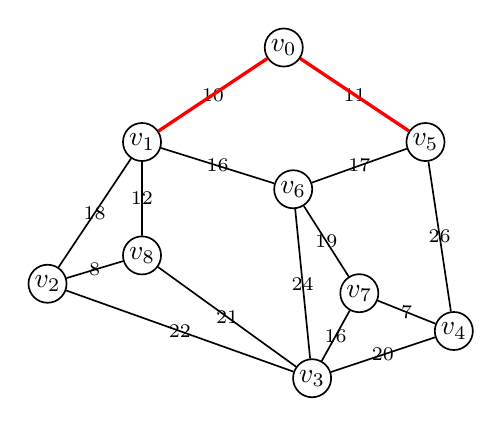
\begin{tikzpicture}[scale=1.2,node distance=2cm,semithick,inner sep=1pt,bend angle=45]
%\draw[help lines] (-3,-3) grid (3,0);
\node[circle,draw] (v0)  at (0,0)   {$v_0$};
\node[circle,draw] (v5)  at (1.5,-1) {$v_5$};
\node[circle,draw] (v1) at (-1.5,-1) {$v_1$};
\node[circle,draw] (v2)  at (-2.5,-2.5)   {$v_2$};
\node[circle,draw] (v8)  at (-1.5,-2.2) {$v_8$};
\node[circle,draw] (v6)  at (0.1,-1.5) {$v_6$};
\node[circle,draw] (v3)  at (0.3,-3.5) {$v_3$};
\node[circle,draw] (v7)  at (0.8,-2.6) {$v_7$};
\node[circle,draw] (v4)  at (1.8,-3.0) {$v_4$};
%%
\path
(v0) edge node{\scriptsize $10$} (v1)
     edge node{\scriptsize $11$} (v5)
(v1) edge node{\scriptsize $18$} (v2)
     edge node{\scriptsize $16$} (v6)
     edge node{\scriptsize $12$} (v8)
(v2) edge node{\scriptsize $8$} (v8)
     edge node{\scriptsize $22$} (v3)
(v3) edge node{\scriptsize $21$} (v8)
     edge node{\scriptsize $24$} (v6)
     edge node{\scriptsize $16$} (v7)
     edge node{\scriptsize $20$} (v4)
(v4) edge node{\scriptsize $7$} (v7)
     edge node{\scriptsize $26$} (v5)
(v5) edge node{\scriptsize $17$} (v6)
(v6) edge node{\scriptsize $19$} (v7);  

\draw[very thick,red](v0)--(v1);
\draw[very thick,red](v0)--(v5);
\end{tikzpicture}

\end{figure}
\end{frame}

\begin{frame}[fragile]\ft{\subsubsecname}
\tf i=2
\lstinputlisting[
language=c,
basicstyle=\ttfamily\scriptsize,
linerange={88-94},
firstnumber=21,
numbers=left,
numberstyle=\tiny,
xleftmargin=0.5em,
]{Chapters/Ch06/Code/adjmatrix/adjmatrix.c} %\pause 

\tf执行前,k=5,  
\begin{lstlisting}[xleftmargin=2em]
  0,  0, 18,INF,INF, 11, 16,INF, 12  (lowcost)
 11,INF,INF,INF, 26,  0, 17,INF,INF  (`第`v_5`行`)
  0,  0,  1,  0,  0,  0,  1,  0,  1  (adjvtx)
\end{lstlisting}  
执行后,
\begin{lstlisting}[xleftmargin=2em]
  0,  0, 18,INF, 26,  0, 16,INF, 12  (lowcost)
  0,  0,  1,  0,  5,  0,  1,  0,  1  (adjvtx)
\end{lstlisting}
\end{frame}


\begin{frame}[fragile]\ft{\subsubsecname}
\tf i=3  
\lstinputlisting[
language=c,
basicstyle=\ttfamily\scriptsize,
linerange={79-87},
firstnumber=12,
numbers=left,
numberstyle=\tiny,
xleftmargin=0.5em,
]{Chapters/Ch06/Code/adjmatrix/adjmatrix.c} %\pause 
执行前,
\begin{lstlisting}[xleftmargin=2em]
  0,  0, 18,INF, 26,  0, 16,INF, 12  (lowcost)
  0,  0,  1,  0,  5,  0,  1,  0,  1  (adjvtx)
\end{lstlisting} %\pause 
执行后,min=12, k=8, adjvtx[8]=1,打印结果为(1,8),表示边$(v_1,v_8)$为最小生成树的第二条边。
\end{frame}


\begin{frame}\ft{\subsubsecname}
\begin{figure}
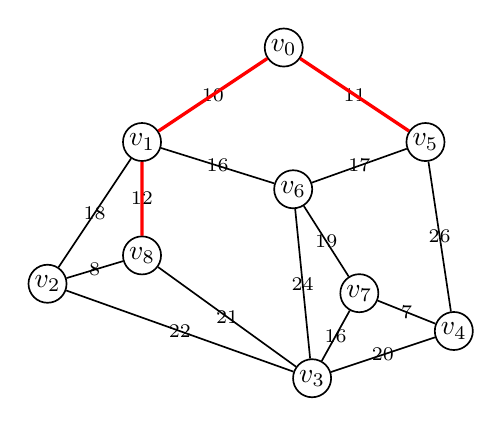
\begin{tikzpicture}[scale=1.2,node distance=2cm,semithick,inner sep=1pt,bend angle=45]
%\draw[help lines] (-3,-3) grid (3,0);
\node[circle,draw] (v0)  at (0,0)   {$v_0$};
\node[circle,draw] (v5)  at (1.5,-1) {$v_5$};
\node[circle,draw] (v1) at (-1.5,-1) {$v_1$};
\node[circle,draw] (v2)  at (-2.5,-2.5)   {$v_2$};
\node[circle,draw] (v8)  at (-1.5,-2.2) {$v_8$};
\node[circle,draw] (v6)  at (0.1,-1.5) {$v_6$};
\node[circle,draw] (v3)  at (0.3,-3.5) {$v_3$};
\node[circle,draw] (v7)  at (0.8,-2.6) {$v_7$};
\node[circle,draw] (v4)  at (1.8,-3.0) {$v_4$};
%%
\path
(v0) edge node{\scriptsize $10$} (v1)
     edge node{\scriptsize $11$} (v5)
(v1) edge node{\scriptsize $18$} (v2)
     edge node{\scriptsize $16$} (v6)
     edge node{\scriptsize $12$} (v8)
(v2) edge node{\scriptsize $8$} (v8)
     edge node{\scriptsize $22$} (v3)
(v3) edge node{\scriptsize $21$} (v8)
     edge node{\scriptsize $24$} (v6)
     edge node{\scriptsize $16$} (v7)
     edge node{\scriptsize $20$} (v4)
(v4) edge node{\scriptsize $7$} (v7)
     edge node{\scriptsize $26$} (v5)
(v5) edge node{\scriptsize $17$} (v6)
(v6) edge node{\scriptsize $19$} (v7);  

\draw[very thick,red](v0)--(v1);
\draw[very thick,red](v0)--(v5);
\draw[very thick,red](v1)--(v8);
\end{tikzpicture}

\end{figure}•
\end{frame}


\begin{frame}[fragile]\ft{\subsubsecname}
\tf i=3 
\lstinputlisting[
language=c,
basicstyle=\ttfamily\scriptsize,
linerange={88-94},
firstnumber=21,
numbers=left,
numberstyle=\tiny,
xleftmargin=0.5em,
]{Chapters/Ch06/Code/adjmatrix/adjmatrix.c} %\pause 

\tf执行前,k=8,  
\begin{lstlisting}[xleftmargin=2em]
  0,  0, 18,INF, 26,  0, 16,INF, 12  (lowcost)
INF, 12,  8, 21,INF,INF,INF,INF,  0  (`第`v_8`行`)
  0,  0,  1,  0,  5,  0,  1,  0,  1  (adjvtx)
\end{lstlisting}  
执行后,
\begin{lstlisting}[xleftmargin=2em]
  0,  0,  8, 21, 26,  0, 16,INF,  0  (lowcost)
  0,  0,  8,  8,  5,  0,  1,  0,  1  (adjvtx)
\end{lstlisting}
\end{frame}


\begin{frame}[fragile]\ft{\subsubsecname}
\tf i=4 
\lstinputlisting[
language=c,
basicstyle=\ttfamily\scriptsize,
linerange={79-87},
firstnumber=12,
numbers=left,
numberstyle=\tiny,
xleftmargin=0.5em,
]{Chapters/Ch06/Code/adjmatrix/adjmatrix.c} %\pause 
执行前,
\begin{lstlisting}[xleftmargin=2em]
  0,  0,  8, 21, 26,  0, 16,INF,  0  (lowcost)
  0,  0,  8,  8,  5,  0,  1,  0,  1  (adjvtx)
\end{lstlisting} %\pause 
执行后,min=8, k=2, adjvtx[2]=8,打印结果为(8,2),表示边$(v_8,v_2)$为最小生成树的第二条边。
\end{frame}


\begin{frame}\ft{\subsubsecname}
\begin{figure}
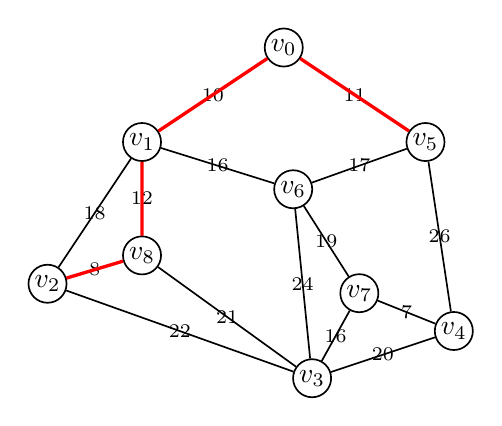
\begin{tikzpicture}[scale=1.2,node distance=2cm,semithick,inner sep=1pt,bend angle=45]
%\draw[help lines] (-3,-3) grid (3,0);
\node[circle,draw] (v0)  at (0,0)   {$v_0$};
\node[circle,draw] (v5)  at (1.5,-1) {$v_5$};
\node[circle,draw] (v1) at (-1.5,-1) {$v_1$};
\node[circle,draw] (v2)  at (-2.5,-2.5)   {$v_2$};
\node[circle,draw] (v8)  at (-1.5,-2.2) {$v_8$};
\node[circle,draw] (v6)  at (0.1,-1.5) {$v_6$};
\node[circle,draw] (v3)  at (0.3,-3.5) {$v_3$};
\node[circle,draw] (v7)  at (0.8,-2.6) {$v_7$};
\node[circle,draw] (v4)  at (1.8,-3.0) {$v_4$};
%%
\path
(v0) edge node{\scriptsize $10$} (v1)
     edge node{\scriptsize $11$} (v5)
(v1) edge node{\scriptsize $18$} (v2)
     edge node{\scriptsize $16$} (v6)
     edge node{\scriptsize $12$} (v8)
(v2) edge node{\scriptsize $8$} (v8)
     edge node{\scriptsize $22$} (v3)
(v3) edge node{\scriptsize $21$} (v8)
     edge node{\scriptsize $24$} (v6)
     edge node{\scriptsize $16$} (v7)
     edge node{\scriptsize $20$} (v4)
(v4) edge node{\scriptsize $7$} (v7)
     edge node{\scriptsize $26$} (v5)
(v5) edge node{\scriptsize $17$} (v6)
(v6) edge node{\scriptsize $19$} (v7);  

\draw[very thick,red](v0)--(v1);
\draw[very thick,red](v0)--(v5);
\draw[very thick,red](v1)--(v8);
\draw[very thick,red](v2)--(v8);
\end{tikzpicture}

\end{figure}•
\end{frame}


\begin{frame}[fragile]\ft{\subsubsecname}
\tf i=4
\lstinputlisting[
language=c,
basicstyle=\ttfamily\scriptsize,
linerange={88-94},
firstnumber=21,
numbers=left,
numberstyle=\tiny,
xleftmargin=0.5em,
]{Chapters/Ch06/Code/adjmatrix/adjmatrix.c} %\pause 

\tf执行前,k=2,  
\begin{lstlisting}[xleftmargin=2em]
  0,  0,  8, 21, 26,  0, 16,INF,  0  (lowcost)
INF,INF,  0, 22,INF,INF,INF,INF,  8  (`第`v_2`行`)
  0,  0,  8,  8,  5,  0,  1,  0,  1  (adjvtx)
\end{lstlisting}  
执行后,
\begin{lstlisting}[xleftmargin=2em]
  0,  0,  0, 21, 26,  0, 16,INF,  0  (lowcost)
  0,  0,  2,  8,  5,  0,  1,  0,  1  (adjvtx)
\end{lstlisting}
\end{frame}


\begin{frame}[fragile]\ft{\subsubsecname}
\tf i=5 
\lstinputlisting[
language=c,
basicstyle=\ttfamily\scriptsize,
linerange={79-87},
firstnumber=12,
numbers=left,
numberstyle=\tiny,
xleftmargin=0.5em,
]{Chapters/Ch06/Code/adjmatrix/adjmatrix.c} %\pause 
执行前,
\begin{lstlisting}[xleftmargin=2em]
  0,  0,  0, 21, 26,  0, 16,INF,  0  (lowcost)
  0,  0,  2,  8,  5,  0,  1,  0,  1  (adjvtx)
\end{lstlisting} %\pause 
执行后,min=16, k=6, adjvtx[6]=1,打印结果为(1,6),表示边$(v_1,v_6)$为最小生成树的第二条边。
\end{frame}


\begin{frame}\ft{\subsubsecname}
\begin{figure}
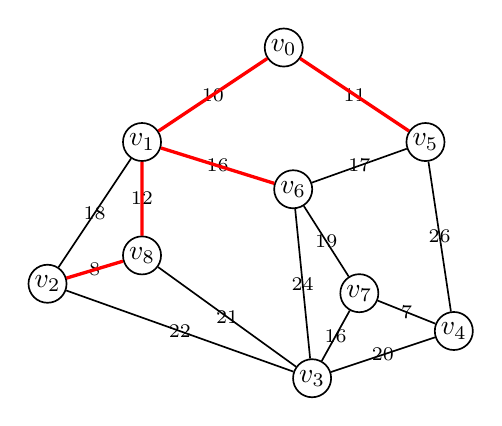
\begin{tikzpicture}[scale=1.2,node distance=2cm,semithick,inner sep=1pt,bend angle=45]
%\draw[help lines] (-3,-3) grid (3,0);
\node[circle,draw] (v0)  at (0,0)   {$v_0$};
\node[circle,draw] (v5)  at (1.5,-1) {$v_5$};
\node[circle,draw] (v1) at (-1.5,-1) {$v_1$};
\node[circle,draw] (v2)  at (-2.5,-2.5)   {$v_2$};
\node[circle,draw] (v8)  at (-1.5,-2.2) {$v_8$};
\node[circle,draw] (v6)  at (0.1,-1.5) {$v_6$};
\node[circle,draw] (v3)  at (0.3,-3.5) {$v_3$};
\node[circle,draw] (v7)  at (0.8,-2.6) {$v_7$};
\node[circle,draw] (v4)  at (1.8,-3.0) {$v_4$};
%%
\path
(v0) edge node{\scriptsize $10$} (v1)
     edge node{\scriptsize $11$} (v5)
(v1) edge node{\scriptsize $18$} (v2)
     edge node{\scriptsize $16$} (v6)
     edge node{\scriptsize $12$} (v8)
(v2) edge node{\scriptsize $8$} (v8)
     edge node{\scriptsize $22$} (v3)
(v3) edge node{\scriptsize $21$} (v8)
     edge node{\scriptsize $24$} (v6)
     edge node{\scriptsize $16$} (v7)
     edge node{\scriptsize $20$} (v4)
(v4) edge node{\scriptsize $7$} (v7)
     edge node{\scriptsize $26$} (v5)
(v5) edge node{\scriptsize $17$} (v6)
(v6) edge node{\scriptsize $19$} (v7);  

\draw[very thick,red](v0)--(v1);
\draw[very thick,red](v0)--(v5);
\draw[very thick,red](v1)--(v8);
\draw[very thick,red](v2)--(v8);
\draw[very thick,red](v1)--(v6);
\end{tikzpicture}

\end{figure}
\end{frame}

\begin{frame}[fragile]\ft{\subsubsecname}
\tf i=5 
\lstinputlisting[
language=c,
basicstyle=\ttfamily\scriptsize,
linerange={88-94},
firstnumber=21,
numbers=left,
numberstyle=\tiny,
xleftmargin=0.5em,
]{Chapters/Ch06/Code/adjmatrix/adjmatrix.c} %\pause 

\tf执行前,k=6,  
\begin{lstlisting}[xleftmargin=2em]
  0,  0,  0, 21, 26,  0, 16,INF,  0  (lowcost)
INF, 16,INF,INF,INF, 17,  0, 19,INF  (`第`v_6`行`)
  0,  0,  2,  8,  5,  0,  1,  0,  1  (adjvtx)
\end{lstlisting}  
执行后,
\begin{lstlisting}[xleftmargin=2em]
  0,  0,  0, 21, 26,  0,  0, 19,  0  (lowcost)
  0,  0,  2,  8,  5,  0,  1,  6,  1  (adjvtx)
\end{lstlisting}
\end{frame}


\begin{frame}[fragile]\ft{\subsubsecname}
\tf i=6  
\lstinputlisting[
language=c,
basicstyle=\ttfamily\scriptsize,
linerange={79-87},
firstnumber=12,
numbers=left,
numberstyle=\tiny,
xleftmargin=0.5em,
]{Chapters/Ch06/Code/adjmatrix/adjmatrix.c} %\pause 
执行前,
\begin{lstlisting}[xleftmargin=2em]
  0,  0,  0, 21, 26,  0,  0, 19,  0  (lowcost)
  0,  0,  2,  8,  5,  0,  1,  6,  1  (adjvtx)
\end{lstlisting} %\pause 
执行后,min=19, k=7, adjvtx[7]=6,打印结果为(7,6),表示边$(v_7,v_6)$为最小生成树的第二条边。
\end{frame}


\begin{frame}\ft{\subsubsecname}
\begin{figure}
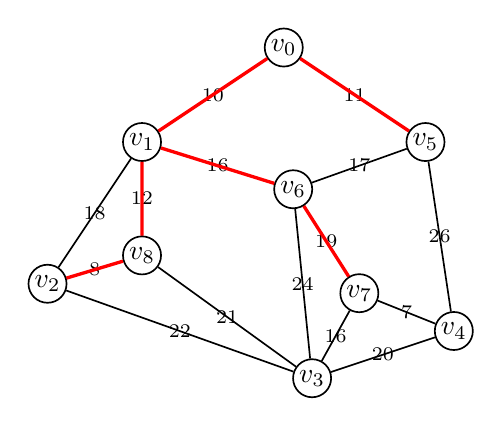
\begin{tikzpicture}[scale=1.2,node distance=2cm,semithick,inner sep=1pt,bend angle=45]
%\draw[help lines] (-3,-3) grid (3,0);
\node[circle,draw] (v0)  at (0,0)   {$v_0$};
\node[circle,draw] (v5)  at (1.5,-1) {$v_5$};
\node[circle,draw] (v1) at (-1.5,-1) {$v_1$};
\node[circle,draw] (v2)  at (-2.5,-2.5)   {$v_2$};
\node[circle,draw] (v8)  at (-1.5,-2.2) {$v_8$};
\node[circle,draw] (v6)  at (0.1,-1.5) {$v_6$};
\node[circle,draw] (v3)  at (0.3,-3.5) {$v_3$};
\node[circle,draw] (v7)  at (0.8,-2.6) {$v_7$};
\node[circle,draw] (v4)  at (1.8,-3.0) {$v_4$};
%%
\path
(v0) edge node{\scriptsize $10$} (v1)
     edge node{\scriptsize $11$} (v5)
(v1) edge node{\scriptsize $18$} (v2)
     edge node{\scriptsize $16$} (v6)
     edge node{\scriptsize $12$} (v8)
(v2) edge node{\scriptsize $8$} (v8)
     edge node{\scriptsize $22$} (v3)
(v3) edge node{\scriptsize $21$} (v8)
     edge node{\scriptsize $24$} (v6)
     edge node{\scriptsize $16$} (v7)
     edge node{\scriptsize $20$} (v4)
(v4) edge node{\scriptsize $7$} (v7)
     edge node{\scriptsize $26$} (v5)
(v5) edge node{\scriptsize $17$} (v6)
(v6) edge node{\scriptsize $19$} (v7);  

\draw[very thick,red](v0)--(v1);
\draw[very thick,red](v0)--(v5);
\draw[very thick,red](v1)--(v8);
\draw[very thick,red](v2)--(v8);
\draw[very thick,red](v1)--(v6);
\draw[very thick,red](v7)--(v6);
\end{tikzpicture}

\end{figure}
\end{frame}


\begin{frame}[fragile]\ft{\subsubsecname}
\tf i=6
\lstinputlisting[
language=c,
basicstyle=\ttfamily\scriptsize,
linerange={88-94},
firstnumber=21,
numbers=left,
numberstyle=\tiny,
xleftmargin=0.5em,
]{Chapters/Ch06/Code/adjmatrix/adjmatrix.c} %\pause 

\tf执行前,k=7,  
\begin{lstlisting}[xleftmargin=2em]
  0,  0,  0, 21, 26,  0,  0, 19,  0  (lowcost)
INF,INF,INF, 16,  7,INF, 19,  0,INF  (`第`v_7`行`)
  0,  0,  2,  8,  5,  0,  1,  6,  1  (adjvtx)
\end{lstlisting}   %\pause 
执行后,
\begin{lstlisting}[xleftmargin=2em]
  0,  0,  0, 16,  7,  0,  0,  0,  0  (lowcost)
  0,  0,  2,  7,  7,  0,  1,  6,  1  (adjvtx)
\end{lstlisting}
\end{frame}


\begin{frame}[fragile]\ft{\subsubsecname}
\tf i=7
\lstinputlisting[
language=c,
basicstyle=\ttfamily\scriptsize,
linerange={79-87},
firstnumber=12,
numbers=left,
numberstyle=\tiny,
xleftmargin=0.5em,
]{Chapters/Ch06/Code/adjmatrix/adjmatrix.c} %\pause 
执行前,
\begin{lstlisting}[xleftmargin=2em]
  0,  0,  0, 16,  7,  0,  0,  0,  0  (lowcost)
  0,  0,  2,  7,  7,  0,  1,  6,  1  (adjvtx)
\end{lstlisting} %\pause 
执行后,min=7, k=4, adjvtx[4]=7,打印结果为(7,4),表示边$(v_7,v_4)$为最小生成树的第二条边。
\end{frame}


\begin{frame}\ft{\subsubsecname}
\begin{figure}
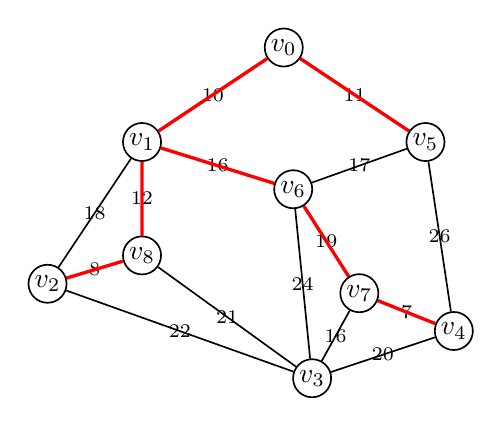
\begin{tikzpicture}[scale=1.2,node distance=2cm,semithick,inner sep=1pt,bend angle=45]
%\draw[help lines] (-3,-3) grid (3,0);
\node[circle,draw] (v0)  at (0,0)   {$v_0$};
\node[circle,draw] (v5)  at (1.5,-1) {$v_5$};
\node[circle,draw] (v1) at (-1.5,-1) {$v_1$};
\node[circle,draw] (v2)  at (-2.5,-2.5)   {$v_2$};
\node[circle,draw] (v8)  at (-1.5,-2.2) {$v_8$};
\node[circle,draw] (v6)  at (0.1,-1.5) {$v_6$};
\node[circle,draw] (v3)  at (0.3,-3.5) {$v_3$};
\node[circle,draw] (v7)  at (0.8,-2.6) {$v_7$};
\node[circle,draw] (v4)  at (1.8,-3.0) {$v_4$};
%%
\path
(v0) edge node{\scriptsize $10$} (v1)
     edge node{\scriptsize $11$} (v5)
(v1) edge node{\scriptsize $18$} (v2)
     edge node{\scriptsize $16$} (v6)
     edge node{\scriptsize $12$} (v8)
(v2) edge node{\scriptsize $8$} (v8)
     edge node{\scriptsize $22$} (v3)
(v3) edge node{\scriptsize $21$} (v8)
     edge node{\scriptsize $24$} (v6)
     edge node{\scriptsize $16$} (v7)
     edge node{\scriptsize $20$} (v4)
(v4) edge node{\scriptsize $7$} (v7)
     edge node{\scriptsize $26$} (v5)
(v5) edge node{\scriptsize $17$} (v6)
(v6) edge node{\scriptsize $19$} (v7);  

\draw[very thick,red](v0)--(v1);
\draw[very thick,red](v0)--(v5);
\draw[very thick,red](v1)--(v8);
\draw[very thick,red](v2)--(v8);
\draw[very thick,red](v1)--(v6);
\draw[very thick,red](v7)--(v6);
\draw[very thick,red](v7)--(v4);
\end{tikzpicture}

\end{figure}
\end{frame}


\begin{frame}[fragile]\ft{\subsubsecname}
\tf i=7 
\lstinputlisting[
language=c,
basicstyle=\ttfamily\scriptsize,
linerange={88-94},
firstnumber=21,
numbers=left,
numberstyle=\tiny,
xleftmargin=0.5em,
]{Chapters/Ch06/Code/adjmatrix/adjmatrix.c} %\pause 

\tf执行前,k=4,  
\begin{lstlisting}[xleftmargin=2em]
  0,  0,  0, 16,  7,  0,  0,  0,  0  (lowcost)
INF,INF,INF, 20,  0, 26,INF,  7,INF  (`第`v_4`行`)
  0,  0,  2,  7,  7,  0,  1,  6,  1  (adjvtx)
\end{lstlisting}  
执行后,
\begin{lstlisting}[xleftmargin=2em]
  0,  0,  0, 16,  0,  0,  0,  0,  0  (lowcost)
  0,  0,  2,  7,  7,  0,  1,  6,  1  (adjvtx)
\end{lstlisting}
\end{frame}


\begin{frame}[fragile]\ft{\subsubsecname}
\tf i=8 
\lstinputlisting[
language=c,
basicstyle=\ttfamily\scriptsize,
linerange={79-87},
firstnumber=12,
numbers=left,
numberstyle=\tiny,
xleftmargin=0.5em,
]{Chapters/Ch06/Code/adjmatrix/adjmatrix.c} %\pause 
执行前,
\begin{lstlisting}[xleftmargin=2em]
  0,  0,  0, 16,  0,  0,  0,  0,  0  (lowcost)
  0,  0,  2,  7,  7,  0,  1,  6,  1  (adjvtx)
\end{lstlisting} %\pause 
执行后,min=16, k=3, adjvtx[3]=7,打印结果为(7,3),表示边$(v_7,v_3)$为最小生成树的第二条边。
\end{frame}


\begin{frame}\ft{\subsubsecname}
\begin{figure}
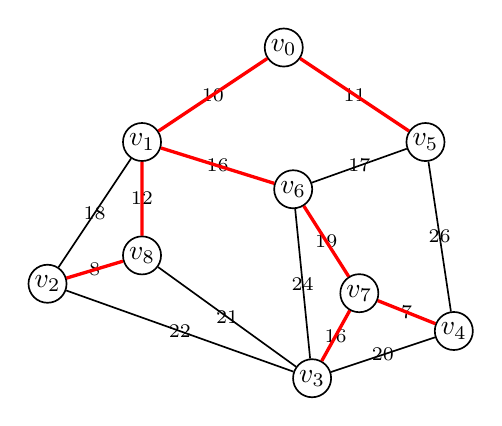
\begin{tikzpicture}[scale=1.2,node distance=2cm,semithick,inner sep=1pt,bend angle=45]
%\draw[help lines] (-3,-3) grid (3,0);
\node[circle,draw] (v0)  at (0,0)   {$v_0$};
\node[circle,draw] (v5)  at (1.5,-1) {$v_5$};
\node[circle,draw] (v1) at (-1.5,-1) {$v_1$};
\node[circle,draw] (v2)  at (-2.5,-2.5)   {$v_2$};
\node[circle,draw] (v8)  at (-1.5,-2.2) {$v_8$};
\node[circle,draw] (v6)  at (0.1,-1.5) {$v_6$};
\node[circle,draw] (v3)  at (0.3,-3.5) {$v_3$};
\node[circle,draw] (v7)  at (0.8,-2.6) {$v_7$};
\node[circle,draw] (v4)  at (1.8,-3.0) {$v_4$};
%%
\path
(v0) edge node{\scriptsize $10$} (v1)
     edge node{\scriptsize $11$} (v5)
(v1) edge node{\scriptsize $18$} (v2)
     edge node{\scriptsize $16$} (v6)
     edge node{\scriptsize $12$} (v8)
(v2) edge node{\scriptsize $8$} (v8)
     edge node{\scriptsize $22$} (v3)
(v3) edge node{\scriptsize $21$} (v8)
     edge node{\scriptsize $24$} (v6)
     edge node{\scriptsize $16$} (v7)
     edge node{\scriptsize $20$} (v4)
(v4) edge node{\scriptsize $7$} (v7)
     edge node{\scriptsize $26$} (v5)
(v5) edge node{\scriptsize $17$} (v6)
(v6) edge node{\scriptsize $19$} (v7);  

\draw[very thick,red](v0)--(v1);
\draw[very thick,red](v0)--(v5);
\draw[very thick,red](v1)--(v8);
\draw[very thick,red](v2)--(v8);
\draw[very thick,red](v1)--(v6);
\draw[very thick,red](v7)--(v6);
\draw[very thick,red](v7)--(v4);
\draw[very thick,red](v7)--(v3);
\end{tikzpicture}

\end{figure}
\end{frame}


\begin{frame}\ft{\subsubsecname}
\tf 设$G=(V,E)$为连通网,$\bar E$为$G$上最小生成树中边的集合。算法从$U=\{u_0\}, u_0\in V, \bar E=\{\}$开始。重复执行以下操作:在所有$u\in U, v\in V/U$的边$(u,v)\in E$中找一条代价最小的边$(u_0,v_0)$并入集合$\bar E$,同时$v_0$并入$U$,直到$U=V$为止。此时$\bar E$中必有$n-1$条边,则$T=(V,\bar E)$为$G$的最小生成树。 \vspace{0.1in}

算法复杂度为$O(n^2)$。
\end{frame}


\subsubsection{\tf Kruskal算法}
\begin{frame}\ft{\subsubsecname}
\tf Kruskal算法直接以边为目标去构建最小生成树。由于权值在边上,直接找最小权值的边构建生成树是很自然的想法,不过构建时需考虑是否会形成环路。
\end{frame}

\begin{frame}\ft{\subsubsecname}
\begin{figure}
\begin{tikzpicture}[scale=1.0,node distance=2cm,semithick,inner sep=1pt,bend angle=45]
%\draw[help lines] (-3,-3) grid (3,0);
\node[circle,draw] (v0)  at (0,0)   {$v_0$};
\node[circle,draw] (v5)  at (1.5,-1) {$v_5$};
\node[circle,draw] (v1) at (-1.5,-1) {$v_1$};
\node[circle,draw] (v2)  at (-2.5,-2.5)   {$v_2$};
\node[circle,draw] (v8)  at (-1.5,-2.2) {$v_8$};
\node[circle,draw] (v6)  at (0.1,-1.5) {$v_6$};
\node[circle,draw] (v3)  at (0.3,-3.5) {$v_3$};
\node[circle,draw] (v7)  at (0.8,-2.6) {$v_7$};
\node[circle,draw] (v4)  at (1.8,-3.0) {$v_4$};
%%
\path
(v0) edge node{\tiny $10$} (v1)
     edge node{\tiny $11$} (v5)
(v1) edge node{\tiny $18$} (v2)
     edge node{\tiny $16$} (v6)
     edge node{\tiny $12$} (v8)
(v2) edge node{\tiny $8$} (v8)
     edge node{\tiny $22$} (v3)
(v3) edge node{\tiny $21$} (v8)
     edge node{\tiny $24$} (v6)
     edge node{\tiny $16$} (v7)
     edge node{\tiny $20$} (v4)
(v4) edge node{\tiny $7$} (v7)
     edge node{\tiny $26$} (v5)
(v5) edge node{\tiny $17$} (v6)
(v6) edge node{\tiny $19$} (v7);  

\matrix (am) at (3,-1) [matrix of nodes,left delimiter=|,right delimiter=|,row sep=0.05pt,column sep=5pt,right] 
  {
      & \tf begin & \tf end & \tf weight \\
    \tf edge[0]  & \tf 4& \tf 7 &  \tf 7\\
    \tf edge[1]  & \tf 2& \tf 8 &  \tf 8\\
    \tf edge[2]  & \tf 0& \tf 1 &  \tf 10\\
    \tf edge[3]  & \tf 0& \tf 5 &  \tf 11\\
    \tf edge[4]  & \tf 1& \tf 8 &  \tf 12\\
    \tf edge[5]  & \tf 3& \tf 7 &  \tf 16\\
    \tf edge[6]  & \tf 1& \tf 6 &  \tf 16\\
    \tf edge[7]  & \tf 5& \tf 6 &  \tf 17\\
    \tf edge[8]  & \tf 1& \tf 2 &  \tf 18\\
    \tf edge[9]  & \tf 6& \tf 7 &  \tf 19\\
    \tf edge[10] & \tf 3& \tf 4 &  \tf 20\\
    \tf edge[11] & \tf 3& \tf 8 &  \tf 21\\
    \tf edge[12] & \tf 2& \tf 3 &  \tf 22\\
    \tf edge[13] & \tf 3& \tf 6 &  \tf 24\\
    \tf edge[14] & \tf 4& \tf 5 &  \tf 26\\
  };            

\end{tikzpicture}

\end{figure}•
\end{frame}

\begin{frame}\ft{\subsubsecname}
\lstinputlisting[
language=c,
basicstyle=\ttfamily\scriptsize,
numbers=left,
numberstyle=\tiny,
xleftmargin=0.5em,
linerange={98-113},
frame=tb,
]{Chapters/Ch06/Code/adjmatrix/adjmatrix.c}
\end{frame}

\begin{frame}\ft{\subsubsecname}
\lstinputlisting[
language=c,
basicstyle=\ttfamily\scriptsize,
numbers=left,
numberstyle=\tiny,
xleftmargin=0.5em,
linerange={115-119},
frame=tb,
]{Chapters/Ch06/Code/adjmatrix/adjmatrix.c}
\end{frame}

\begin{frame}\ft{\subsubsecname}
\tf  
\lstinputlisting[
language=c,
basicstyle=\ttfamily\scriptsize,
linerange={101-103},
firstnumber=4,
numbers=left,
numberstyle=\tiny,
xleftmargin=0.5em,
]{Chapters/Ch06/Code/adjmatrix/adjmatrix.c} %\pause 
定义数组parent,并初始化为0。
\end{frame}


\begin{frame}[fragile]\ft{\subsubsecname}
\tf i=0
\lstinputlisting[
language=c,
basicstyle=\ttfamily\scriptsize,
linerange={104-112},
firstnumber=7,
numbers=left,
numberstyle=\tiny,
xleftmargin=0.5em,
]{Chapters/Ch06/Code/adjmatrix/adjmatrix.c} %\pause 
\vspace{0.05in}


第8行:调用Find,传入parent和边$(v_4,v_7)$的begin:4,返回n=4。 \vspace{0.05in}%\pause

第9行:调用Find,传入parent和边$(v_4,v_7)$的end:7,返回m=7。 \vspace{0.05in} %\pause 

第10-14行:因n!=m,故parent[4]=7,此时
\begin{lstlisting}[xleftmargin=2em]
0, 0, 0, 0, 7, 0, 0, 0, 0
\end{lstlisting}
打印结果为(4,7) 7,将边$(v_4,v_7)$纳入到最小生成树中。
\end{frame}

\begin{frame}\ft{\subsubsecname}
\begin{figure}
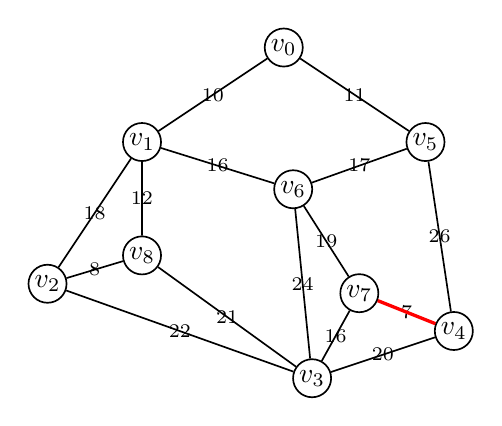
\begin{tikzpicture}[scale=1.2,node distance=2cm,semithick,inner sep=1pt,bend angle=45]
%\draw[help lines] (-3,-3) grid (3,0);
\node[circle,draw] (v0)  at (0,0)   {$v_0$};
\node[circle,draw] (v5)  at (1.5,-1) {$v_5$};
\node[circle,draw] (v1) at (-1.5,-1) {$v_1$};
\node[circle,draw] (v2)  at (-2.5,-2.5)   {$v_2$};
\node[circle,draw] (v8)  at (-1.5,-2.2) {$v_8$};
\node[circle,draw] (v6)  at (0.1,-1.5) {$v_6$};
\node[circle,draw] (v3)  at (0.3,-3.5) {$v_3$};
\node[circle,draw] (v7)  at (0.8,-2.6) {$v_7$};
\node[circle,draw] (v4)  at (1.8,-3.0) {$v_4$};
%%
\path
(v0) edge node{\scriptsize $10$} (v1)
     edge node{\scriptsize $11$} (v5)
(v1) edge node{\scriptsize $18$} (v2)
     edge node{\scriptsize $16$} (v6)
     edge node{\scriptsize $12$} (v8)
(v2) edge node{\scriptsize $8$} (v8)
     edge node{\scriptsize $22$} (v3)
(v3) edge node{\scriptsize $21$} (v8)
     edge node{\scriptsize $24$} (v6)
     edge node{\scriptsize $16$} (v7)
     edge node{\scriptsize $20$} (v4)
(v4) edge node{\scriptsize $7$} (v7)
     edge node{\scriptsize $26$} (v5)
(v5) edge node{\scriptsize $17$} (v6)
(v6) edge node{\scriptsize $19$} (v7);  

\draw[very thick,red](v4)--(v7);

\end{tikzpicture}

\end{figure}
\end{frame}


\begin{frame}[fragile]\ft{\subsubsecname}
\tf i=1
\lstinputlisting[
language=c,
basicstyle=\ttfamily\scriptsize,
linerange={104-112},
firstnumber=7,
numbers=left,
numberstyle=\tiny,
xleftmargin=0.5em,
]{Chapters/Ch06/Code/adjmatrix/adjmatrix.c} %\pause 
\vspace{0.05in}

第8行:调用Find,传入parent和边$(v_2,v_8)$的begin:2,返回n=2。 \vspace{0.05in}

第9行:调用Find,传入parent和边$(v_2,v_8)$的end:8,返回m=8。 \vspace{0.05in}

第10-14行:因n!=m,故parent[2]=8,此时
\begin{lstlisting}[xleftmargin=2em]
0, 0, 8, 0, 7, 0, 0, 0, 0
\end{lstlisting}
打印结果为(2,8) 8,将边$(v_2,v_8)$纳入到最小生成树中。
\end{frame}

\begin{frame}\ft{\subsubsecname}
\begin{figure}
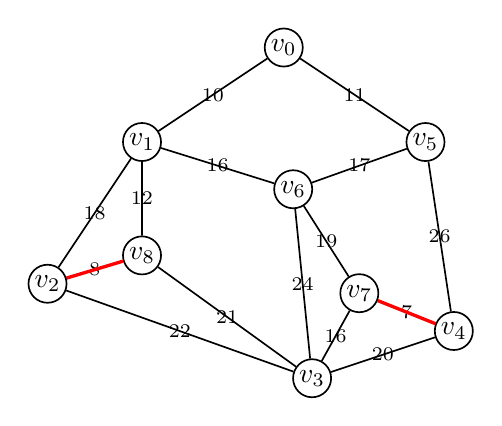
\begin{tikzpicture}[scale=1.2,node distance=2cm,semithick,inner sep=1pt,bend angle=45]
%\draw[help lines] (-3,-3) grid (3,0);
\node[circle,draw] (v0)  at (0,0)   {$v_0$};
\node[circle,draw] (v5)  at (1.5,-1) {$v_5$};
\node[circle,draw] (v1) at (-1.5,-1) {$v_1$};
\node[circle,draw] (v2)  at (-2.5,-2.5)   {$v_2$};
\node[circle,draw] (v8)  at (-1.5,-2.2) {$v_8$};
\node[circle,draw] (v6)  at (0.1,-1.5) {$v_6$};
\node[circle,draw] (v3)  at (0.3,-3.5) {$v_3$};
\node[circle,draw] (v7)  at (0.8,-2.6) {$v_7$};
\node[circle,draw] (v4)  at (1.8,-3.0) {$v_4$};
%%
\path
(v0) edge node{\scriptsize $10$} (v1)
     edge node{\scriptsize $11$} (v5)
(v1) edge node{\scriptsize $18$} (v2)
     edge node{\scriptsize $16$} (v6)
     edge node{\scriptsize $12$} (v8)
(v2) edge node{\scriptsize $8$} (v8)
     edge node{\scriptsize $22$} (v3)
(v3) edge node{\scriptsize $21$} (v8)
     edge node{\scriptsize $24$} (v6)
     edge node{\scriptsize $16$} (v7)
     edge node{\scriptsize $20$} (v4)
(v4) edge node{\scriptsize $7$} (v7)
     edge node{\scriptsize $26$} (v5)
(v5) edge node{\scriptsize $17$} (v6)
(v6) edge node{\scriptsize $19$} (v7);  

\draw[very thick,red](v4)--(v7);
\draw[very thick,red](v2)--(v8);
\end{tikzpicture}

\end{figure}
\end{frame}

\begin{frame}[fragile]\ft{\subsubsecname}
\tf i=2
\lstinputlisting[
language=c,
basicstyle=\ttfamily\scriptsize,
linerange={104-112},
firstnumber=7,
numbers=left,
numberstyle=\tiny,
xleftmargin=0.5em,
]{Chapters/Ch06/Code/adjmatrix/adjmatrix.c} %\pause 
\vspace{0.05in}

第8行:调用Find,传入parent和边$(v_0,v_1)$的begin:0,返回n=0。 \vspace{0.05in}

第9行:调用Find,传入parent和边$(v_0,v_1)$的end:1,返回m=1。 \vspace{0.05in}

第10-14行:因n!=m,故parent[0]=1,此时
\begin{lstlisting}[xleftmargin=2em]
1, 0, 8, 0, 7, 0, 0, 0, 0
\end{lstlisting}
打印结果为(0,1) 10,将边$(v_0,v_1)$纳入到最小生成树中。
\end{frame}

\begin{frame}\ft{\subsubsecname}
\begin{figure}
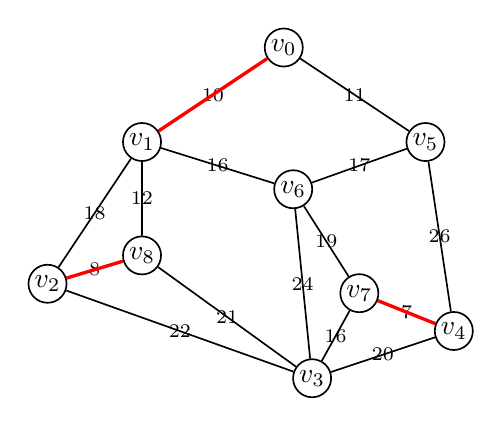
\begin{tikzpicture}[scale=1.2,node distance=2cm,semithick,inner sep=1pt,bend angle=45]
%\draw[help lines] (-3,-3) grid (3,0);
\node[circle,draw] (v0)  at (0,0)   {$v_0$};
\node[circle,draw] (v5)  at (1.5,-1) {$v_5$};
\node[circle,draw] (v1) at (-1.5,-1) {$v_1$};
\node[circle,draw] (v2)  at (-2.5,-2.5)   {$v_2$};
\node[circle,draw] (v8)  at (-1.5,-2.2) {$v_8$};
\node[circle,draw] (v6)  at (0.1,-1.5) {$v_6$};
\node[circle,draw] (v3)  at (0.3,-3.5) {$v_3$};
\node[circle,draw] (v7)  at (0.8,-2.6) {$v_7$};
\node[circle,draw] (v4)  at (1.8,-3.0) {$v_4$};
%%
\path
(v0) edge node{\scriptsize $10$} (v1)
     edge node{\scriptsize $11$} (v5)
(v1) edge node{\scriptsize $18$} (v2)
     edge node{\scriptsize $16$} (v6)
     edge node{\scriptsize $12$} (v8)
(v2) edge node{\scriptsize $8$} (v8)
     edge node{\scriptsize $22$} (v3)
(v3) edge node{\scriptsize $21$} (v8)
     edge node{\scriptsize $24$} (v6)
     edge node{\scriptsize $16$} (v7)
     edge node{\scriptsize $20$} (v4)
(v4) edge node{\scriptsize $7$} (v7)
     edge node{\scriptsize $26$} (v5)
(v5) edge node{\scriptsize $17$} (v6)
(v6) edge node{\scriptsize $19$} (v7);  

\draw[very thick,red](v4)--(v7);
\draw[very thick,red](v2)--(v8);
\draw[very thick,red](v0)--(v1);
\end{tikzpicture}

\end{figure}
\end{frame}


\begin{frame}[fragile]\ft{\subsubsecname}
\tf i=3
\lstinputlisting[
language=c,
basicstyle=\ttfamily\scriptsize,
linerange={104-112},
firstnumber=7,
numbers=left,
numberstyle=\tiny,
xleftmargin=0.5em,
]{Chapters/Ch06/Code/adjmatrix/adjmatrix.c} %\pause 
\vspace{0.05in}

第8行:调用Find,传入parent和边$(v_0,v_5)$的begin:0,返回n=1。 \vspace{0.05in}

第9行:调用Find,传入parent和边$(v_0,v_5)$的end:5,返回m=5。 \vspace{0.05in}

第10-14行:因n!=m,故parent[1]=5,此时
\begin{lstlisting}[xleftmargin=2em]
1, 5, 8, 0, 7, 0, 0, 0, 0
\end{lstlisting}
打印结果为(0,5) 11,将边$(v_0,v_5)$纳入到最小生成树中。
\end{frame}

\begin{frame}\ft{\subsubsecname}
\begin{figure}
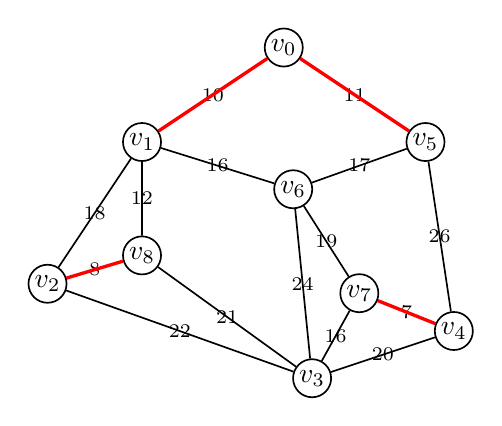
\begin{tikzpicture}[scale=1.2,node distance=2cm,semithick,inner sep=1pt,bend angle=45]
%\draw[help lines] (-3,-3) grid (3,0);
\node[circle,draw] (v0)  at (0,0)   {$v_0$};
\node[circle,draw] (v5)  at (1.5,-1) {$v_5$};
\node[circle,draw] (v1) at (-1.5,-1) {$v_1$};
\node[circle,draw] (v2)  at (-2.5,-2.5)   {$v_2$};
\node[circle,draw] (v8)  at (-1.5,-2.2) {$v_8$};
\node[circle,draw] (v6)  at (0.1,-1.5) {$v_6$};
\node[circle,draw] (v3)  at (0.3,-3.5) {$v_3$};
\node[circle,draw] (v7)  at (0.8,-2.6) {$v_7$};
\node[circle,draw] (v4)  at (1.8,-3.0) {$v_4$};
%%
\path
(v0) edge node{\scriptsize $10$} (v1)
     edge node{\scriptsize $11$} (v5)
(v1) edge node{\scriptsize $18$} (v2)
     edge node{\scriptsize $16$} (v6)
     edge node{\scriptsize $12$} (v8)
(v2) edge node{\scriptsize $8$} (v8)
     edge node{\scriptsize $22$} (v3)
(v3) edge node{\scriptsize $21$} (v8)
     edge node{\scriptsize $24$} (v6)
     edge node{\scriptsize $16$} (v7)
     edge node{\scriptsize $20$} (v4)
(v4) edge node{\scriptsize $7$} (v7)
     edge node{\scriptsize $26$} (v5)
(v5) edge node{\scriptsize $17$} (v6)
(v6) edge node{\scriptsize $19$} (v7);  

\draw[very thick,red](v4)--(v7);
\draw[very thick,red](v2)--(v8);
\draw[very thick,red](v0)--(v1);
\draw[very thick,red](v0)--(v5);
\end{tikzpicture}

\end{figure}
\end{frame}



\begin{frame}[fragile]\ft{\subsubsecname}
\tf i=4
\lstinputlisting[
language=c,
basicstyle=\ttfamily\scriptsize,
linerange={104-112},
firstnumber=7,
numbers=left,
numberstyle=\tiny,
xleftmargin=0.5em,
]{Chapters/Ch06/Code/adjmatrix/adjmatrix.c} %\pause 
\vspace{0.05in}

第8行:调用Find,传入parent和边$(v_1,v_8)$的begin:1,返回n=5。 \vspace{0.05in}

第9行:调用Find,传入parent和边$(v_1,v_8)$的end:8,返回m=8。 \vspace{0.05in}

第10-14行:因n!=m,故parent[5]=8,此时
\begin{lstlisting}[xleftmargin=2em]
1, 5, 8, 0, 7, 8, 0, 0, 0
\end{lstlisting}
打印结果为(1,8) 12,将边$(v_1,v_8)$纳入到最小生成树中。
\end{frame}

\begin{frame}\ft{\subsubsecname}
\begin{figure}
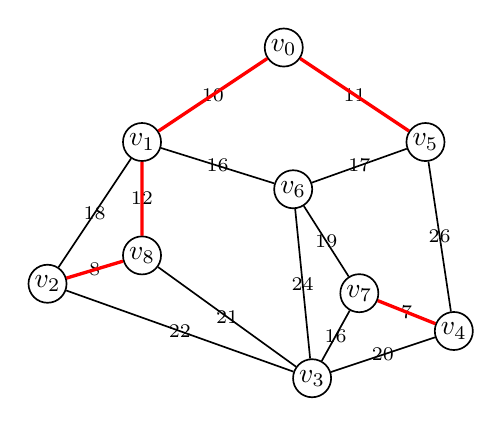
\begin{tikzpicture}[scale=1.2,node distance=2cm,semithick,inner sep=1pt,bend angle=45]
%\draw[help lines] (-3,-3) grid (3,0);
\node[circle,draw] (v0)  at (0,0)   {$v_0$};
\node[circle,draw] (v5)  at (1.5,-1) {$v_5$};
\node[circle,draw] (v1) at (-1.5,-1) {$v_1$};
\node[circle,draw] (v2)  at (-2.5,-2.5)   {$v_2$};
\node[circle,draw] (v8)  at (-1.5,-2.2) {$v_8$};
\node[circle,draw] (v6)  at (0.1,-1.5) {$v_6$};
\node[circle,draw] (v3)  at (0.3,-3.5) {$v_3$};
\node[circle,draw] (v7)  at (0.8,-2.6) {$v_7$};
\node[circle,draw] (v4)  at (1.8,-3.0) {$v_4$};
%%
\path
(v0) edge node{\scriptsize $10$} (v1)
     edge node{\scriptsize $11$} (v5)
(v1) edge node{\scriptsize $18$} (v2)
     edge node{\scriptsize $16$} (v6)
     edge node{\scriptsize $12$} (v8)
(v2) edge node{\scriptsize $8$} (v8)
     edge node{\scriptsize $22$} (v3)
(v3) edge node{\scriptsize $21$} (v8)
     edge node{\scriptsize $24$} (v6)
     edge node{\scriptsize $16$} (v7)
     edge node{\scriptsize $20$} (v4)
(v4) edge node{\scriptsize $7$} (v7)
     edge node{\scriptsize $26$} (v5)
(v5) edge node{\scriptsize $17$} (v6)
(v6) edge node{\scriptsize $19$} (v7);  

\draw[very thick,red](v4)--(v7);
\draw[very thick,red](v2)--(v8);
\draw[very thick,red](v0)--(v1);
\draw[very thick,red](v0)--(v5);
\draw[very thick,red](v1)--(v8);
\end{tikzpicture}

\end{figure}
\end{frame}


\begin{frame}[fragile]\ft{\subsubsecname}
\tf i=5
\lstinputlisting[
language=c,
basicstyle=\ttfamily\scriptsize,
linerange={104-112},
firstnumber=7,
numbers=left,
numberstyle=\tiny,
xleftmargin=0.5em,
]{Chapters/Ch06/Code/adjmatrix/adjmatrix.c} %\pause 
\vspace{0.05in}

第8行:调用Find,传入parent和边$(v_3,v_7)$的begin:3,返回n=3。 \vspace{0.05in}

第9行:调用Find,传入parent和边$(v_3,v_7)$的end:7,返回m=7。 \vspace{0.05in}

第10-14行:因n!=m,故parent[3]=7,此时
\begin{lstlisting}[xleftmargin=2em]
1, 5, 8, 7, 7, 8, 0, 0, 0
\end{lstlisting}
打印结果为(3,7) 16,将边$(v_3,v_7)$纳入到最小生成树中。
\end{frame}

\begin{frame}\ft{\subsubsecname}
\begin{figure}
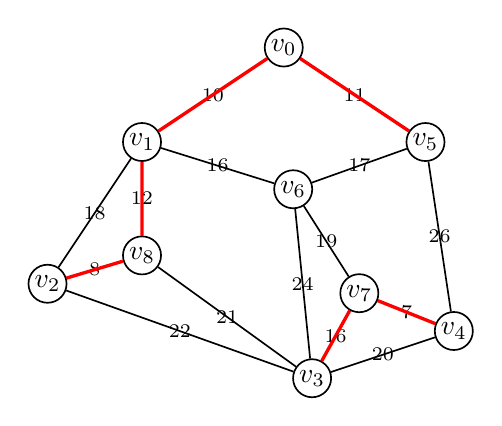
\begin{tikzpicture}[scale=1.2,node distance=2cm,semithick,inner sep=1pt,bend angle=45]
%\draw[help lines] (-3,-3) grid (3,0);
\node[circle,draw] (v0)  at (0,0)   {$v_0$};
\node[circle,draw] (v5)  at (1.5,-1) {$v_5$};
\node[circle,draw] (v1) at (-1.5,-1) {$v_1$};
\node[circle,draw] (v2)  at (-2.5,-2.5)   {$v_2$};
\node[circle,draw] (v8)  at (-1.5,-2.2) {$v_8$};
\node[circle,draw] (v6)  at (0.1,-1.5) {$v_6$};
\node[circle,draw] (v3)  at (0.3,-3.5) {$v_3$};
\node[circle,draw] (v7)  at (0.8,-2.6) {$v_7$};
\node[circle,draw] (v4)  at (1.8,-3.0) {$v_4$};
%%
\path
(v0) edge node{\scriptsize $10$} (v1)
     edge node{\scriptsize $11$} (v5)
(v1) edge node{\scriptsize $18$} (v2)
     edge node{\scriptsize $16$} (v6)
     edge node{\scriptsize $12$} (v8)
(v2) edge node{\scriptsize $8$} (v8)
     edge node{\scriptsize $22$} (v3)
(v3) edge node{\scriptsize $21$} (v8)
     edge node{\scriptsize $24$} (v6)
     edge node{\scriptsize $16$} (v7)
     edge node{\scriptsize $20$} (v4)
(v4) edge node{\scriptsize $7$} (v7)
     edge node{\scriptsize $26$} (v5)
(v5) edge node{\scriptsize $17$} (v6)
(v6) edge node{\scriptsize $19$} (v7);  

\draw[very thick,red](v4)--(v7);
\draw[very thick,red](v2)--(v8);
\draw[very thick,red](v0)--(v1);
\draw[very thick,red](v0)--(v5);
\draw[very thick,red](v1)--(v8);
\draw[very thick,red](v3)--(v7);
\end{tikzpicture}

\end{figure}
\end{frame}


\begin{frame}[fragile]\ft{\subsubsecname}
\tf i=6
\lstinputlisting[
language=c,
basicstyle=\ttfamily\scriptsize,
linerange={104-112},
firstnumber=7,
numbers=left,
numberstyle=\tiny,
xleftmargin=0.5em,
]{Chapters/Ch06/Code/adjmatrix/adjmatrix.c} %\pause 
\vspace{0.05in}

第8行:调用Find,传入parent和边$(v_1,v_6)$的begin:1,返回n=8。 \vspace{0.05in}

第9行:调用Find,传入parent和边$(v_1,v_6)$的end:6,返回m=6。 \vspace{0.05in}

第10-14行:因n!=m,故parent[8]=6,此时
\begin{lstlisting}[xleftmargin=2em]
1, 5, 8, 7, 7, 8, 0, 0, 6
\end{lstlisting}
打印结果为(1,6) 16,将边$(v_1,v_6)$纳入到最小生成树中。
\end{frame}

\begin{frame}\ft{\subsubsecname}
\begin{figure}
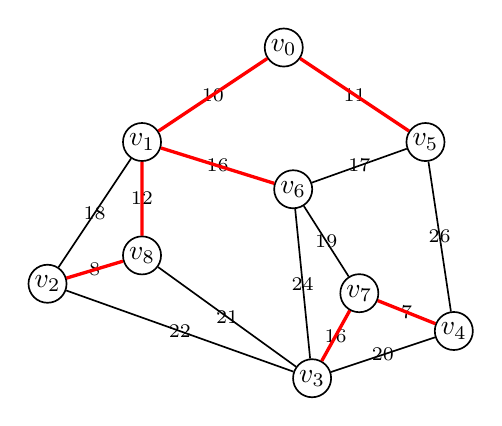
\begin{tikzpicture}[scale=1.2,node distance=2cm,semithick,inner sep=1pt,bend angle=45]
%\draw[help lines] (-3,-3) grid (3,0);
\node[circle,draw] (v0)  at (0,0)   {$v_0$};
\node[circle,draw] (v5)  at (1.5,-1) {$v_5$};
\node[circle,draw] (v1) at (-1.5,-1) {$v_1$};
\node[circle,draw] (v2)  at (-2.5,-2.5)   {$v_2$};
\node[circle,draw] (v8)  at (-1.5,-2.2) {$v_8$};
\node[circle,draw] (v6)  at (0.1,-1.5) {$v_6$};
\node[circle,draw] (v3)  at (0.3,-3.5) {$v_3$};
\node[circle,draw] (v7)  at (0.8,-2.6) {$v_7$};
\node[circle,draw] (v4)  at (1.8,-3.0) {$v_4$};
%%
\path
(v0) edge node{\scriptsize $10$} (v1)
     edge node{\scriptsize $11$} (v5)
(v1) edge node{\scriptsize $18$} (v2)
     edge node{\scriptsize $16$} (v6)
     edge node{\scriptsize $12$} (v8)
(v2) edge node{\scriptsize $8$} (v8)
     edge node{\scriptsize $22$} (v3)
(v3) edge node{\scriptsize $21$} (v8)
     edge node{\scriptsize $24$} (v6)
     edge node{\scriptsize $16$} (v7)
     edge node{\scriptsize $20$} (v4)
(v4) edge node{\scriptsize $7$} (v7)
     edge node{\scriptsize $26$} (v5)
(v5) edge node{\scriptsize $17$} (v6)
(v6) edge node{\scriptsize $19$} (v7);  

\draw[very thick,red](v4)--(v7);
\draw[very thick,red](v2)--(v8);
\draw[very thick,red](v0)--(v1);
\draw[very thick,red](v0)--(v5);
\draw[very thick,red](v1)--(v8);
\draw[very thick,red](v3)--(v7);
\draw[very thick,red](v1)--(v6);
\end{tikzpicture}

\end{figure}
\end{frame}


\begin{frame}[fragile]\ft{\subsubsecname}
\tf i=7 
\lstinputlisting[
language=c,
basicstyle=\ttfamily\scriptsize,
linerange={104-112},
firstnumber=7,
numbers=left,
numberstyle=\tiny,
xleftmargin=0.5em,
]{Chapters/Ch06/Code/adjmatrix/adjmatrix.c} %\pause 
\vspace{0.05in}

第8行:调用Find,传入parent和边$(v_5,v_6)$的begin:5,返回n=6。 \vspace{0.05in}

第9行:调用Find,传入parent和边$(v_5,v_6)$的end:6,返回m=6。 \vspace{0.05in}

第10-14行:因n==m,不打印,继续下一循环。此时边$(v_5,v_6)$导致形成回路。
\end{frame}


\begin{frame}[fragile]\ft{\subsubsecname}
\tf i=8 
\lstinputlisting[
language=c,
basicstyle=\ttfamily\scriptsize,
linerange={104-112},
firstnumber=7,
numbers=left,
numberstyle=\tiny,
xleftmargin=0.5em,
]{Chapters/Ch06/Code/adjmatrix/adjmatrix.c} %\pause 
\vspace{0.05in}

第8行:调用Find,传入parent和边$(v_1,v_2)$的begin:1,返回n=6。 \vspace{0.05in}

第9行:调用Find,传入parent和边$(v_1,v_2)$的end:2,返回m=6。 \vspace{0.05in}

第10-14行:因n==m,不打印,继续下一循环。此时边$(v_1,v_2)$导致形成回路。
\end{frame}


\begin{frame}[fragile]\ft{\subsubsecname}
\tf i=9 
\lstinputlisting[
language=c,
basicstyle=\ttfamily\scriptsize,
linerange={104-112},
firstnumber=7,
numbers=left,
numberstyle=\tiny,
xleftmargin=0.5em,
]{Chapters/Ch06/Code/adjmatrix/adjmatrix.c} %\pause 
\vspace{0.05in}

第8行:调用Find,传入parent和边$(v_6,v_7)$的begin:6,返回n=6。 \vspace{0.05in}

第9行:调用Find,传入parent和边$(v_6,v_7)$的end:7,返回m=7。 \vspace{0.05in}

第10-14行:因n!=m,故parent[6]=7,此时
\begin{lstlisting}[xleftmargin=2em]
1, 5, 8, 7, 7, 8, 7, 0, 6
\end{lstlisting}
打印结果为(6,7) 19,将边$(v_6,v_7)$纳入到最小生成树中。

\end{frame}


\begin{frame}\ft{\subsubsecname}
\begin{figure}
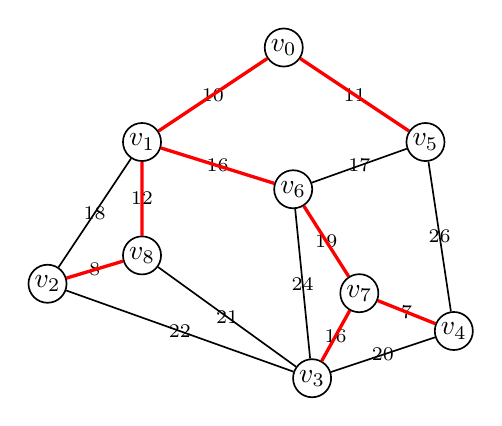
\begin{tikzpicture}[scale=1.2,node distance=2cm,semithick,inner sep=1pt,bend angle=45]
%\draw[help lines] (-3,-3) grid (3,0);
\node[circle,draw] (v0)  at (0,0)   {$v_0$};
\node[circle,draw] (v5)  at (1.5,-1) {$v_5$};
\node[circle,draw] (v1) at (-1.5,-1) {$v_1$};
\node[circle,draw] (v2)  at (-2.5,-2.5)   {$v_2$};
\node[circle,draw] (v8)  at (-1.5,-2.2) {$v_8$};
\node[circle,draw] (v6)  at (0.1,-1.5) {$v_6$};
\node[circle,draw] (v3)  at (0.3,-3.5) {$v_3$};
\node[circle,draw] (v7)  at (0.8,-2.6) {$v_7$};
\node[circle,draw] (v4)  at (1.8,-3.0) {$v_4$};
%%
\path
(v0) edge node{\scriptsize $10$} (v1)
     edge node{\scriptsize $11$} (v5)
(v1) edge node{\scriptsize $18$} (v2)
     edge node{\scriptsize $16$} (v6)
     edge node{\scriptsize $12$} (v8)
(v2) edge node{\scriptsize $8$} (v8)
     edge node{\scriptsize $22$} (v3)
(v3) edge node{\scriptsize $21$} (v8)
     edge node{\scriptsize $24$} (v6)
     edge node{\scriptsize $16$} (v7)
     edge node{\scriptsize $20$} (v4)
(v4) edge node{\scriptsize $7$} (v7)
     edge node{\scriptsize $26$} (v5)
(v5) edge node{\scriptsize $17$} (v6)
(v6) edge node{\scriptsize $19$} (v7);  

\draw[very thick,red](v4)--(v7);
\draw[very thick,red](v2)--(v8);
\draw[very thick,red](v0)--(v1);
\draw[very thick,red](v0)--(v5);
\draw[very thick,red](v1)--(v8);
\draw[very thick,red](v3)--(v7);
\draw[very thick,red](v1)--(v6);
\draw[very thick,red](v6)--(v7);
\end{tikzpicture}

\end{figure}
\end{frame}


\begin{frame}[fragile]\ft{\subsubsecname}
\tf i=10
\lstinputlisting[
language=c,
basicstyle=\ttfamily\scriptsize,
linerange={104-112},
firstnumber=7,
numbers=left,
numberstyle=\tiny,
xleftmargin=0.5em,
]{Chapters/Ch06/Code/adjmatrix/adjmatrix.c} %\pause 
\vspace{0.05in}

第8行:调用Find,传入parent和边$(v_3,v_4)$的begin:3,返回n=7。 \vspace{0.05in}

第9行:调用Find,传入parent和边$(v_3,v_4)$的end:4,返回m=7。 \vspace{0.05in}

第10-14行:因n==m,不打印,继续下一循环。此时边$(v_3,v_4)$导致形成回路。
\end{frame}

\begin{frame}[fragile]\ft{\subsubsecname}
\tf i=11
\lstinputlisting[
language=c,
basicstyle=\ttfamily\scriptsize,
linerange={104-112},
firstnumber=7,
numbers=left,
numberstyle=\tiny,
xleftmargin=0.5em,
]{Chapters/Ch06/Code/adjmatrix/adjmatrix.c} %\pause 
\vspace{0.05in}

第8行:调用Find,传入parent和边$(v_3,v_8)$的begin:3,返回n=7。 \vspace{0.05in}

第9行:调用Find,传入parent和边$(v_3,v_8)$的end:8,返回m=7。 \vspace{0.05in}

第10-14行:因n==m,不打印,继续下一循环。此时边$(v_3,v_8)$导致形成回路。
\end{frame}


\begin{frame}[fragile]\ft{\subsubsecname}
\tf i=12
\lstinputlisting[
language=c,
basicstyle=\ttfamily\scriptsize,
linerange={104-112},
firstnumber=7,
numbers=left,
numberstyle=\tiny,
xleftmargin=0.5em,
]{Chapters/Ch06/Code/adjmatrix/adjmatrix.c} %\pause 
\vspace{0.05in}

第8行:调用Find,传入parent和边$(v_3,v_6)$的begin:3,返回n=7。 \vspace{0.05in}

第9行:调用Find,传入parent和边$(v_3,v_6)$的end:6,返回m=7。 \vspace{0.05in}

第10-14行:因n==m,不打印,继续下一循环。此时边$(v_3,v_6)$导致形成回路。
\end{frame}




\begin{frame}[fragile]\ft{\subsubsecname}
\tf i=12
\lstinputlisting[
language=c,
basicstyle=\ttfamily\scriptsize,
linerange={104-112},
firstnumber=7,
numbers=left,
numberstyle=\tiny,
xleftmargin=0.5em,
]{Chapters/Ch06/Code/adjmatrix/adjmatrix.c} %\pause 
\vspace{0.05in}

第8行:调用Find,传入parent和边$(v_4,v_5)$的begin:4,返回n=7。 \vspace{0.05in}

第9行:调用Find,传入parent和边$(v_4,v_5)$的end:5,返回m=7。 \vspace{0.05in}

第10-14行:因n==m,不打印,继续下一循环。此时边$(v_4,v_5)$导致形成回路。
\end{frame}


\begin{frame}\ft{\subsubsecname}
设$G=(V,E)$是连通网,令最小生成树的初始状态为只有$n$个顶点但无边的非连通图$T=(V,\{\})$,图中每个顶点自成一个连通分量。在$E$中选择代价最小的边,若该边依附的顶点落在$T$中不同的连通分量上,则将此边加入到$T$中,否则舍去此边而选择下一条代价最小的边。依次类推,直到$T$中所有顶点都在同一连通分量上为止。
%\pause
\vspace{0.1in}

时间复杂度为$O(e\log e)$。

\end{frame}

%% \begin{frame}\ft{\subsubsecname}

%% \end{frame}

%% \begin{frame}\ft{\subsubsecname}

%% \end{frame}

%% \begin{frame}\ft{\subsubsecname}

%% \end{frame}

%% \begin{frame}\ft{\subsubsecname}

%% \end{frame}
